\documentclass{../exhibit}
\usepackage{pgfplots}

\title{Slide (off the Plank) Rules}

%% Font
\usepackage{imfellEnglish}
\usepackage[T1]{fontenc}
\raggedright

\usepackage{background}

\backgroundsetup{
scale=1,
color=black,
opacity=0.4,
angle=0,
contents={%
  \includegraphics[height=\paperheight]{mapBackground.jpg}%%https://upload.wikimedia.org/wikipedia/commons/8/81/Nautical_chart_of_the_West_Indies_1797.jpg
  }%
}




%% For the context
%% https://tex.stackexchange.com/questions/86150/torn-page-effect/86151#86151
\usepackage{tikz}
\usetikzlibrary{decorations.pathmorphing}
\definecolor{paper}{RGB}{239,227,157}





\renewcommand{\maketitle}{ %
  \begin{center}
    \scalebox{8}{\thetitle}
  \end{center}
  
\begin{tabular*}{\textwidth}{c @{\extracolsep{\fill}} c}  
\resizebox{4in}{!}{\begin{minipage}[b]{3in}\huge\directions\end{minipage}} &
  \resizebox{4in}{!}{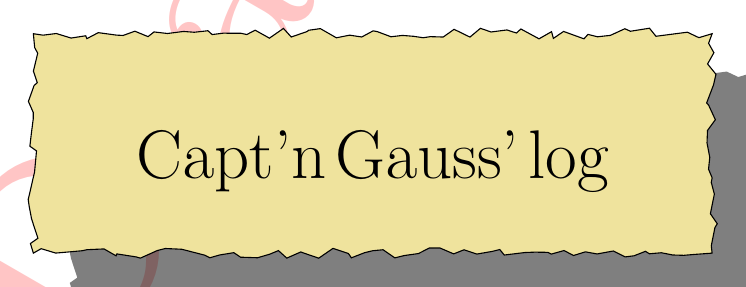
\begin{tikzpicture}[pencildraw/.style={ %
    decorate,
    decoration={random steps,segment length=4pt,amplitude=2pt}
    } %
]
\node[
preaction={fill=black,opacity=.5,transform canvas={xshift=.5cm,yshift=-.5cm}},
pencildraw,draw,fill=paper,text width=3in,inner sep=.5cm] 
{\begin{center}\Huge Capt'n Gauss' log \end{center}\vspace{.7cm} {\huge\context}};
\end{tikzpicture}}

\end{tabular*}

\vfill

\includegraphics[width=3in]{logoPirate.png}\hfill \includegraphics[width=2in]{bammLogo.png}


}


\begin{document}

\begin{context} We put the ``slide rule'' to the test today in a raid on a
merchant vessel. The ease and speed of calculations allowed us to
outmaneuver the enemy and escape with a bountiful haul. The crew is
already showing a marked improvement in their mathematical abilities,
and morale is high.
\end{context}

\begin{directions}
  Use the provided slide rules to multiply numbers.
\end{directions}

\begin{example}
You can add numbers by placing two rulers next to each other.
  \begin{center}
  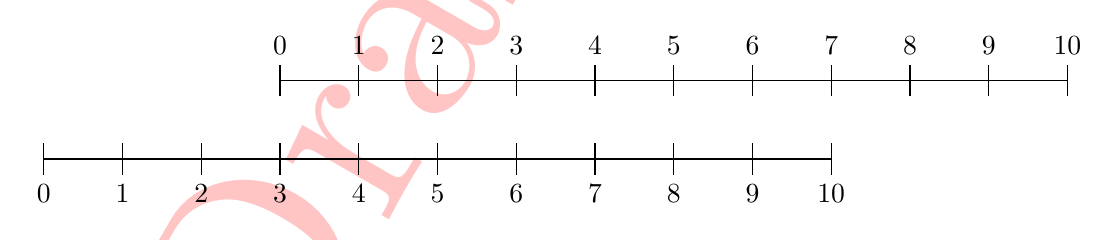
\begin{tikzpicture}

% Draw the first ruler
\draw (0,0) -- (10,0); % Draw the main line
\foreach \x in {0,1,...,10} {  % Draw tick marks
    \draw (\x,-0.2) -- (\x,0.2);
    \node[below] at (\x,-0.2) {\x}; % Add numbers
}

\begin{scope}[shift={(3,0)}]

% Draw the second ruler
\draw (0,1) -- (10,1); % Draw the main line
\foreach \x in {0,1,...,10} {  % Draw tick marks
    \draw (\x,0.8) -- (\x,1.2);
    \node[above] at (\x,1.2) {\x}; % Add numbers
}

\end{scope}
\end{tikzpicture}
\end{center}
By putting the ruler marks at different locations, you can produce ``rulers'' that you can use to multiply.
  \begin{center}
  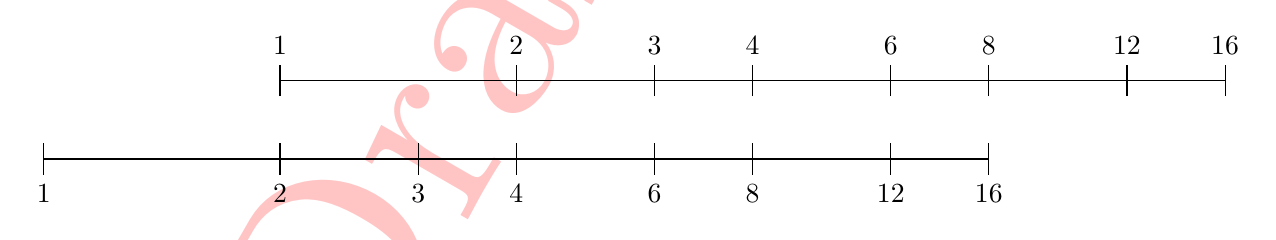
\begin{tikzpicture}

% Draw the first ruler
\draw (0,0) -- (12,0); % Draw the main line
\foreach \x in {1,2,3,4,6,8,12,16} {  % Draw tick marks
    \draw ({3*ln(\x)/ln(2)},-0.2) -- ({3*ln(\x)/ln(2)},0.2);
    \node[below] at ({3*ln(\x)/ln(2)},-0.2) {\x}; % Add numbers
}

\begin{scope}[shift={(3,0)}]

% Draw the second ruler
\draw (0,1) -- (12,1); % Draw the main line
\foreach \x in {1,2,3,4,6,8,12,16} {  % Draw tick marks
    \draw ({3*ln(\x)/ln(2)},0.8) -- ({3*ln(\x)/ln(2)},1.2);
    \node[above] at ({3*ln(\x)/ln(2)},1.2) {\x}; % Add numbers
}

\end{scope}
\end{tikzpicture}
\end{center}
\end{example}

\begin{mathConnections}
  https://bartsnapp.github.io/Math-Outreach-Exhibits/sliderules/
\end{mathConnections}
\end{document}
